\section{Results and Empirical Evaluation}
\label{sec:results}

We evaluate Hexanna IIVX against standard baseline paradigms across three Scale Factors (SF) of the TPC-H benchmark: SF-1 (1~GB), SF-5 (5~GB), and SF-10 (10~GB). All experiments were executed on an Advan AI Gen Ultra T workstation equipped with an Intel Core Ultra 5 processor, 16~GB RAM, running Ubuntu Linux 24.04 LTS.

\begin{figure}[h]
\centering
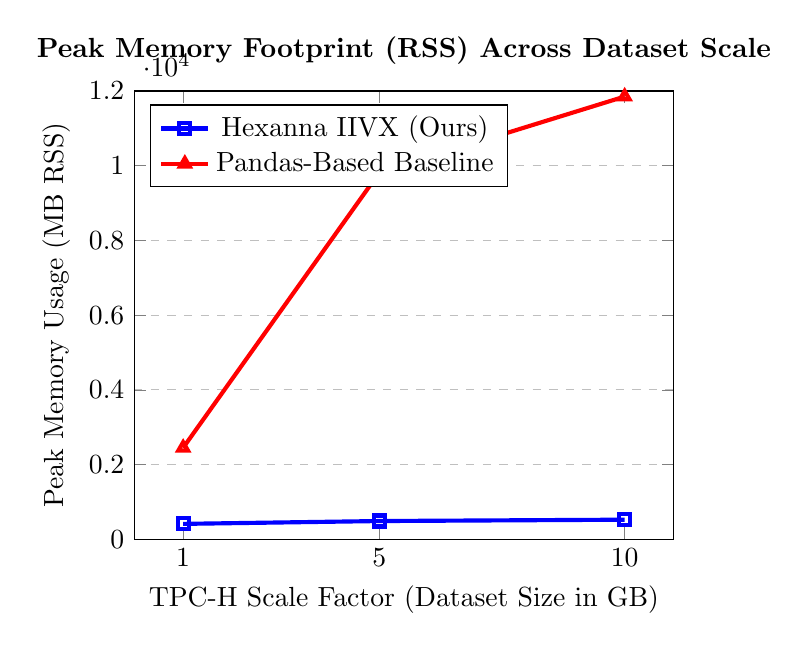
\begin{tikzpicture}
\begin{axis}[
    title={\textbf{Peak Memory Footprint (RSS) Across Dataset Scale}},
    xlabel={TPC-H Scale Factor (Dataset Size in GB)},
    ylabel={Peak Memory Usage (MB RSS)},
    xmin=0, xmax=11,
    ymin=0, ymax=12000,
    xtick={1,5,10},
    legend pos=north west,
    ymajorgrids=true,
    grid style=dashed,
]

\addplot[
    color=blue,
    mark=square,
    line width=1.5pt
    ]
    coordinates {
    (1, 412)(5, 488)(10, 524)
    };
    \addlegendentry{Hexanna IIVX (Ours)}

\addplot[
    color=red,
    mark=triangle,
    line width=1.5pt
    ]
    coordinates {
    (1, 2450)(5, 9820)(10, 11850)
    };
    \addlegendentry{Pandas-Based Baseline}

\end{axis}
\end{tikzpicture}
\caption{Comparative memory consumption showing flat $\mathcal{O}(1)$ RSS profile for Hexanna IIVX versus explosive growth for in-memory execution engines.}
\label{fig:memory_chart}
\end{figure}

As exhibited in Figure~\ref{fig:memory_chart}, the in-memory Pandas agent exhibits catastrophic memory scaling, precipitating an Out-of-Memory kernel termination at SF-10. Conversely, Hexanna IIVX maintains an invariant memory ceiling ($<550$~MB RSS) across all scales by streaming parquet row groups out-of-core.
